\documentclass[12pt]{article}
% set tiems new roman in latex
\usepackage{newtxtext}
\usepackage[paper=letterpaper,margin=2.54cm]{geometry}
\usepackage{amsmath}
\usepackage{amssymb}
\usepackage{amsfonts}
\usepackage{newtxtext, newtxmath}
% \usepackage{enumitem}
\usepackage{enumerate}
\usepackage{titling}
\usepackage[colorlinks=true]{hyperref}
\usepackage{graphicx}
\usepackage{float}
\usepackage{listings}
\usepackage{xcolor}
\usepackage{color}
\usepackage{caption}
\usepackage{subfigure}
\usepackage{float}
\usepackage{booktabs}
\usepackage{multirow}

% citation
\usepackage[numbers]{natbib}



\setlength{\droptitle}{-6em}
% Enter the specific assignment number and topic of that assignment below, and replace "Your Name" with your actual name.
\title{Project: Comp 6771 Image Processing}
\author{Yunqi Xu 40130514}
\date{\today}


\begin{document}
% \maketitle
\begin{titlepage}
  \rule{\textwidth}{1pt}   % The top horizontal rule
    \vspace{0.2\textheight}  % Whitespace between top horizontal rule and title

    %------------------------------------------------------------
    %    Title
    %------------------------------------------------------------

    {\Huge Project: A Study Of Bilateral Filtering}

    \vspace{0.025\textheight}   % Whitespace between the title and short horizontal rule

    \rule{0.83\textwidth}{0.4pt}  % The short horizontal rule under title

    \vspace{0.1\textheight}  % Whitespace between the short horizontal rule and author

    %------------------------------------------------------------
    %    Author
    %------------------------------------------------------------

    {\Large Student name: \textsc{Yunqi Xu}}
    \vfill
    {\Large Student id: 40130514}
    \vfill  % Whitespace between author and date

    {\large \today}
    \vspace{0.1\textheight}  % Whitespace between date and bottom horizontal rule

    %------------------------------------------------------------
    %    Bottom rules
    %------------------------------------------------------------

    \rule{\textwidth}{1pt}  % The bottom horizontal rule
\end{titlepage}

\section{Bilateral filter and Gaussian adaptive bilateral filter}
% \subsection{Bilateral filter and Gaussian adaptive bilateral filter}
\label{section review bilateral}
% overall summary of bilateral filter
Bilateral filter(BF in the following) is an edge-preserving, noise-removing, simple and non-iterative, color-suitable filtering proposed by Tomasi in 1998~\cite{paper_bf}.
The purpose of BF solves the problem of the blurred edges when filtering with a Gaussian low-pass filter, and the unstable output brought by iterative Diffusion methods.

The BF is consisted of the weighted sum of the multiplication of two gaussian-like filters, as shown in fig.~\ref{processing_bf}, where the Domain filter $c(\xi, x) = e^{-\frac{1}{2}(\frac{d(\xi, x)}{\sigma_{d}})^2}$  calculate the Euclidean distance between $\xi$ and $x$, and the Range filter $s(\xi, x) = e^{-\frac{1}{2}(\frac{\delta(f(\xi), f(x))}{\sigma_{r}})^{2}}$ calculate the difference between two intensity values.
By using BF, a noised image could be successfully smoothed, and at the same time, edges in this image could be preserved, as indicated in ~\cite{paper_bf}. 
The paper also mentions that BF is suitable for a color image. 
However, the evaluation of the paper lacks a quantitive comparison with the benchmark.
Also, the smooth is not clean enough since the range kernel generated in BF is a noisy kernel~\cite{paper_gabf}.

\begin{figure}[H]
  \centering
  \subfigure[Processing of Bilateral filter]{
  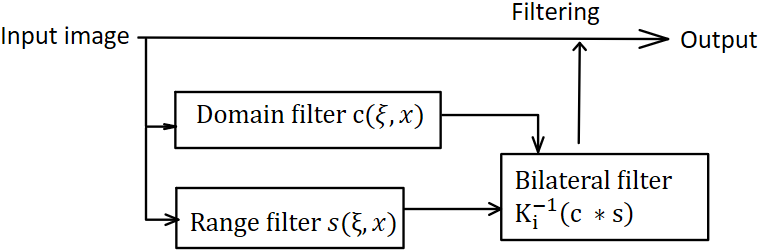
\includegraphics[width=7.5cm]{cite images/1.png}
  % \caption{fig1}
  \label{processing_bf}
  }
  \quad
  \subfigure[Processing Gaussian adaptive bilaterl filter]{
  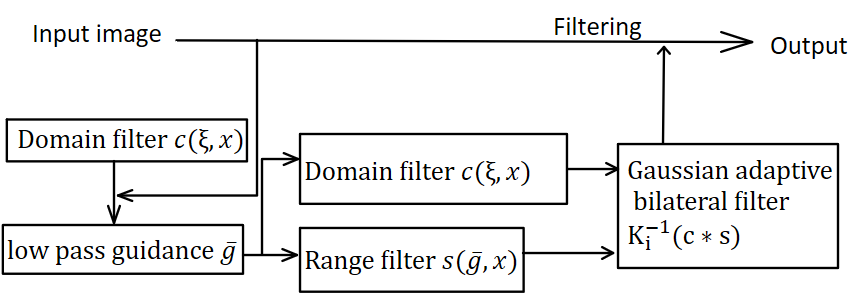
\includegraphics[width=7.5cm]{cite images/2.png}
  \label{processing_gabf}
  }
\caption{Comparison between Bilateral filter and Gaussian adaptive Bilater filter}
\label{processing}
\end{figure}

For solving the problem mentioned above, the Gaussian adaptive bilateral filter(GABF in the following) which is a variation format of BF  is published in 2020~\cite{paper_gabf}.
The GABF can reduce the influence of the noised-contained range filter by two non-identical filters. 

The same as Bf, GABF calculates the weighted sum of the multiplication of two gaussian filters, however, the range filter is generated from the input image with domain filter as shown in~\ref{processing_gabf}.
So, the range filter in GABF comes from the low-pass guidance $\bar{g}$.
The result in~\cite{paper_gabf} indicates the success of the GABF. 
The author uses some popular evaluation methods assess GABF, BF, and some other variations of BF on some public datasets. 
As the result mentions, all of these three evaluation methods prove that the GABF can optimize input image better than others methods.


\bibliographystyle{IEEEtranN}
\bibliography{reference}
% \printbibliography


\clearpage
\section{Experiment}
\label{section Experiment}
% modify with citation of sections

For a better understanding Bilateral filter, we will re-implement the Bilateral filter using python and present the result in this section.
We will present the result on both gray and color images in Section~\ref{subsection reimplement}.
In section~\ref{subsection baseline comparison}, we will use PSNR as the evaluation criteria to compare the re-implement Bilateral filter with other baseline low-pass filter methods to prove the benefit of the Bilateral filter.


\subsection{Experiment result of the Re-implement algorithm}
\label{subsection reimplement}
The main purpose of this section is to provide an improvement of the success of the re-implement of the Bilateral filter.
During our experiment, the input images including all images come from the Bilateral filter paper~\cite{paper_bf} and some others from the internet. 
we will input the same parameters as the original paper suggested. 
In the end, we compared ours with the outputs printed on paper, and also compare with the output from the OpenCV-python official build-in function. 
All of this output indicates the success of our re-implement algorithm. 
We presented the results of the gray images in Section.~\ref{subsubsection test gray} and colorful image in Section.~\ref{subsubsection color images}.


\subsubsection{Experiment result of gray images}
\label{subsubsection test gray}


\begin{figure}[H]
  \centering
  \subfigure[$\sigma_d=1, \sigma_r=10$]{
  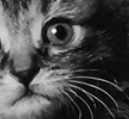
\includegraphics[width=3cm]{output_image/cat_part_ds1_rs10.png}
  % \caption{fig1}
  \label{im_cateye_1_10}
  }
  \quad
  \subfigure[$\sigma_d=1, \sigma_r=30$]{
  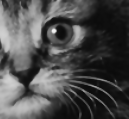
\includegraphics[width=3cm]{output_image/cat_part_ds1_rs30.png}
  }
  \quad
  \subfigure[$\sigma_d=1, \sigma_r=100$]{
  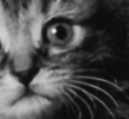
\includegraphics[width=3cm]{output_image/cat_part_ds1_rs100.png}
  }
  \quad
  \subfigure[$\sigma_d=1, \sigma_r=300$]{
  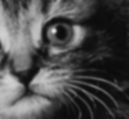
\includegraphics[width=3cm]{output_image/cat_part_ds1_rs300.png}
  }

  \subfigure[$\sigma_d=3, \sigma_r=10$]{
  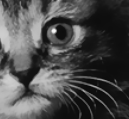
\includegraphics[width=3cm]{output_image/cat_part_ds3_rs10.png}
  % \caption{fig1}
  }
  \quad
  \subfigure[$\sigma_d=3, \sigma_r=30$]{
  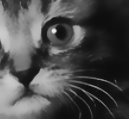
\includegraphics[width=3cm]{output_image/cat_part_ds3_rs30.png}
  }
  \quad
  \subfigure[$\sigma_d=3, \sigma_r=100$]{
  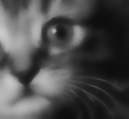
\includegraphics[width=3cm]{output_image/cat_part_ds3_rs100.png}
  }
  \quad
  \subfigure[$\sigma_d=3, \sigma_r=300$]{
  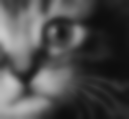
\includegraphics[width=3cm]{output_image/cat_part_ds3_rs300.png}
  }

  \subfigure[$\sigma_d=10, \sigma_r=10$]{
  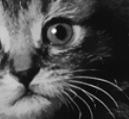
\includegraphics[width=3cm]{output_image/cat_part_ds10_rs10.png}
  % \caption{fig1}
  }
  \quad
  \subfigure[$\sigma_d=10, \sigma_r=30$]{
  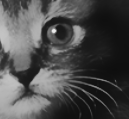
\includegraphics[width=3cm]{output_image/cat_part_ds10_rs30.png}
  }
  \quad
  \subfigure[$\sigma_d=10, \sigma_r=100$]{
  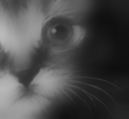
\includegraphics[width=3cm]{output_image/cat_part_ds10_rs100.png}
  }
  \quad
  \subfigure[$\sigma_d=10, \sigma_r=300$]{
  
\includegraphics[width=3cm]{output_image/cat_part_ds10_rs300.png}
  \label{im_cateye_10_300}
  }
\caption{A detail of cat processed with bilateral filters with various range and domain parameter values}
\label{im_cateye}
\end{figure}

Fig.~\ref{im_cateye} presents the output of our re-implement Bilateral filter. 
In our experiment, the $kernel\_size = 23$ is a fixed value through all our filtering. 
We choose the permutations of parameters $\sigma_d = (1, 3, 10)$ and $\sigma_r = (10, 30, 100, 300)$ forming parameter pairs. 
The smooth result of the re-implement Buialteral filter achieves a very similar result compared with Figure 3 from the Bilateral filter paper.
Fig.~\ref{im_cateye_1_10} has the cleanest result, but part of the small noises remain in the image. 
On the other hand, Fig.~\ref{im_cateye_10_300} is the most ambiguous one in these outputs.
It only remains a faint profile of the cat. 

As a comparison, we also input the image with the same parameter pairs into the built-in OpenCV-python function to explore whether it will have the same output as our code. Fig.~\ref{py_cateye} proves the results are similar. 


\begin{figure}[H]
  \centering
  \subfigure[$\sigma_d=1, \sigma_r=10$]{
  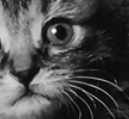
\includegraphics[width=3cm]{output_image_python/cat_part_ds1_rs10.png}
  % \caption{fig1}
  }
  \quad
  \subfigure[$\sigma_d=1, \sigma_r=30$]{
  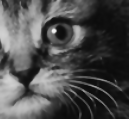
\includegraphics[width=3cm]{output_image_python/cat_part_ds1_rs30.png}
  }
  \quad
  \subfigure[$\sigma_d=1, \sigma_r=100$]{
  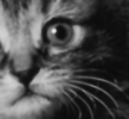
\includegraphics[width=3cm]{output_image_python/cat_part_ds1_rs100.png}
  }
  \quad
  \subfigure[$\sigma_d=1, \sigma_r=300$]{
  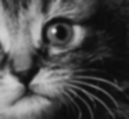
\includegraphics[width=3cm]{output_image_python/cat_part_ds1_rs300.png}
  }

  \subfigure[$\sigma_d=3, \sigma_r=10$]{
  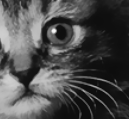
\includegraphics[width=3cm]{output_image_python/cat_part_ds3_rs10.png}
  % \caption{fig1}
  }
  \quad
  \subfigure[$\sigma_d=3, \sigma_r=30$]{
  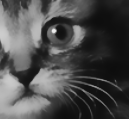
\includegraphics[width=3cm]{output_image_python/cat_part_ds3_rs30.png}
  }
  \quad
  \subfigure[$\sigma_d=3, \sigma_r=100$]{
  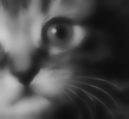
\includegraphics[width=3cm]{output_image_python/cat_part_ds3_rs100.png}
  }
  \quad
  \subfigure[$\sigma_d=3, \sigma_r=300$]{
  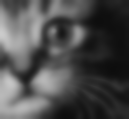
\includegraphics[width=3cm]{output_image_python/cat_part_ds3_rs300.png}
  }

  \subfigure[$\sigma_d=10, \sigma_r=10$]{
  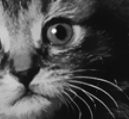
\includegraphics[width=3cm]{output_image_python/cat_part_ds10_rs10.png}
  % \caption{fig1}
  }
  \quad
  \subfigure[$\sigma_d=10, \sigma_r=30$]{
  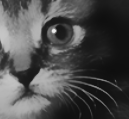
\includegraphics[width=3cm]{output_image_python/cat_part_ds10_rs30.png}
  }
  \quad
  \subfigure[$\sigma_d=10, \sigma_r=100$]{
  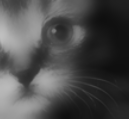
\includegraphics[width=3cm]{output_image_python/cat_part_ds10_rs100.png}
  }
  \quad
  \subfigure[$\sigma_d=10, \sigma_r=300$]{
  
\includegraphics[width=3cm]{output_image_python/cat_part_ds10_rs300.png}
  }
  \caption{A detail figure with bilateral filters with various range and domain parameter values by Opencv python}
  \label{py_cateye}
  \end{figure}

Fig.~\ref{im_cat_large} presents the filtering result between the original input image and the output with parameter $\sigma_d = 3$ and $\sigma_r = 30$. 
The output is very similar to Figure 5 in the Bilateral filter paper.
Also,  The property of edge-preserving is shown in these images, the Kitten's whiskers are preserved after filtering.

\begin{figure}[H]
  \centering
  \subfigure[$\sigma_d=1, \sigma_r=10$]{
  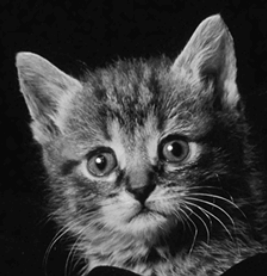
\includegraphics[width=5cm]{original_paper_images/gray/cat.png}
  \label{im_cat_large_original}
  % \caption{fig1}
  }
  \quad
  \subfigure[$\sigma_d=3, \sigma_r=30$]{
  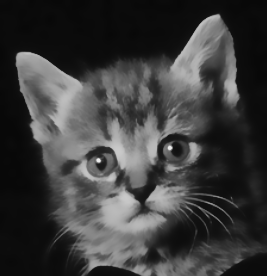
\includegraphics[width=5cm]{output_image/cat_ds3_rs30.png}
  }
  \caption{Output of cat}
  \label{im_cat_large}
  \end{figure}



\begin{figure}[H]
  \centering
  \subfigure[$\sigma_d=1, \sigma_r=10$]{
  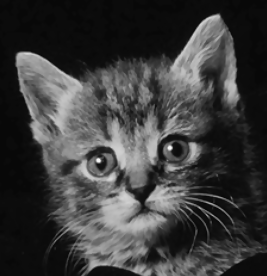
\includegraphics[width=3.5cm]{output_image/cat_ds1_rs10.png}
  % \caption{fig1}
  }
  \quad
  \subfigure[$\sigma_d=1, \sigma_r=30$]{
  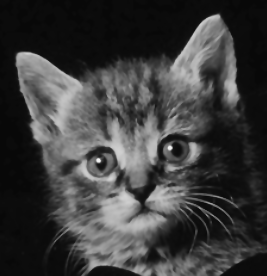
\includegraphics[width=3.5cm]{output_image/cat_ds1_rs30.png}
  }
  \quad
  \subfigure[$\sigma_d=1, \sigma_r=100$]{
  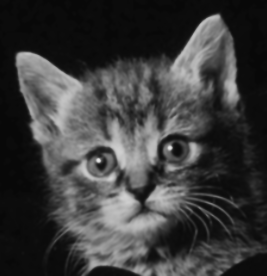
\includegraphics[width=3.5cm]{output_image/cat_ds1_rs100.png}
  }
  \quad
  \subfigure[$\sigma_d=1, \sigma_r=300$]{
  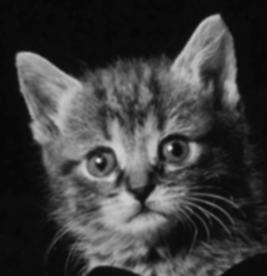
\includegraphics[width=3.5cm]{output_image/cat_ds1_rs300.png}
  }

  \subfigure[$\sigma_d=3, \sigma_r=10$]{
  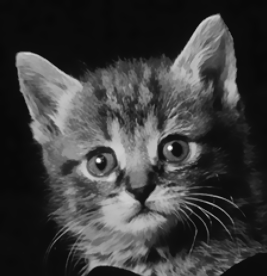
\includegraphics[width=3.5cm]{output_image/cat_ds3_rs10.png}
  % \caption{fig1}
  }
  \quad
  \subfigure[$\sigma_d=3, \sigma_r=30$]{
  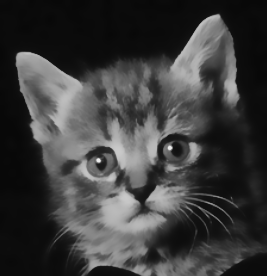
\includegraphics[width=3.5cm]{output_image/cat_ds3_rs30.png}
  }
  \quad
  \subfigure[$\sigma_d=3, \sigma_r=100$]{
  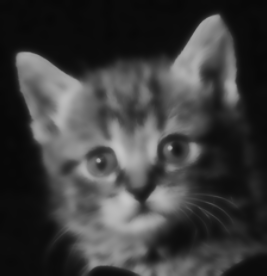
\includegraphics[width=3.5cm]{output_image/cat_ds3_rs100.png}
  }
  \quad
  \subfigure[$\sigma_d=3, \sigma_r=300$]{
  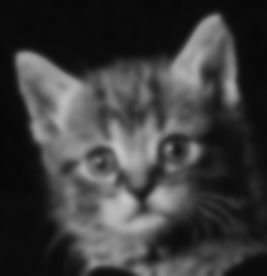
\includegraphics[width=3.5cm]{output_image/cat_ds3_rs300.png}
  }

  \subfigure[$\sigma_d=10, \sigma_r=10$]{
  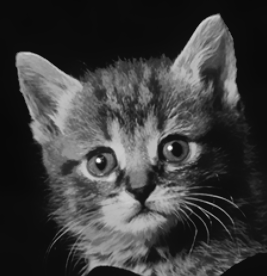
\includegraphics[width=3.5cm]{output_image/cat_ds10_rs10.png}
  % \caption{fig1}
  }
  \quad
  \subfigure[$\sigma_d=10, \sigma_r=30$]{
  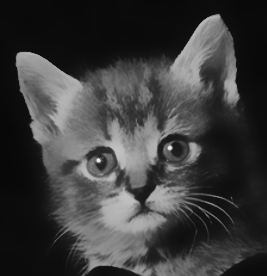
\includegraphics[width=3.5cm]{output_image/cat_ds10_rs30.png}
  }
  \quad
  \subfigure[$\sigma_d=10, \sigma_r=100$]{
  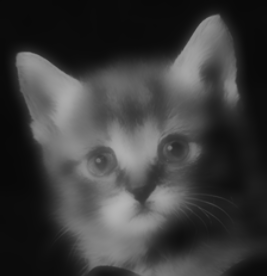
\includegraphics[width=3.5cm]{output_image/cat_ds10_rs100.png}
  }
  \quad
  \subfigure[$\sigma_d=10, \sigma_r=300$]{
  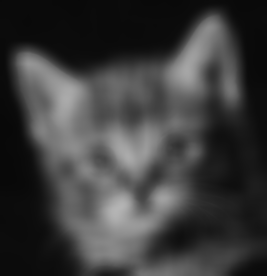
\includegraphics[width=3.5cm]{output_image/cat_ds10_rs300.png}
  }
  \caption{A detail figure with bilateral filters with various range and domain parameter values by re-implement code of cat}
  \label{im_cat}
  \end{figure}

Fig.~\ref{im_cat} are the whole output of the input image ~\ref{im_cat_large_original} with the same parameter pairs as before.

% Fig.~\ref{im_cat} are also two image which prove the success of our re-implement code. 


\begin{figure}[H]
  \centering
  \subfigure[Original snack]{
  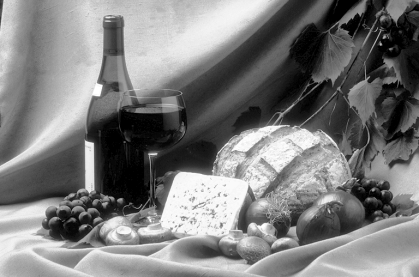
\includegraphics[width=6cm]{original_paper_images/gray/snack_a.png}
  \label{snack_original}
  }
  \quad
  \subfigure[Smoothed snack]{
  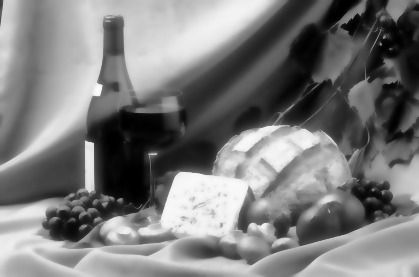
\includegraphics[width=6cm]{output_image/snack_a_ds2_rs50.png}
  \label{snack_original_smooth}
  }
  \quad
  \subfigure[Original Onion]{
  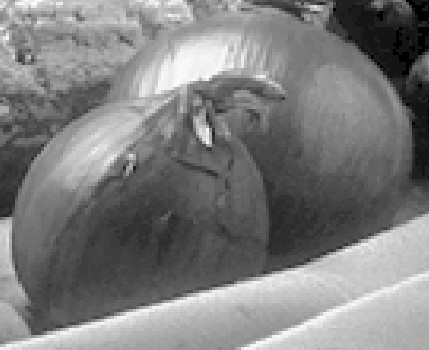
\includegraphics[width=4.5cm]{original_paper_images/gray/onion.png}
  \label{snack_onion}
  }
  \quad
  \subfigure[Smoothed Onion]{
  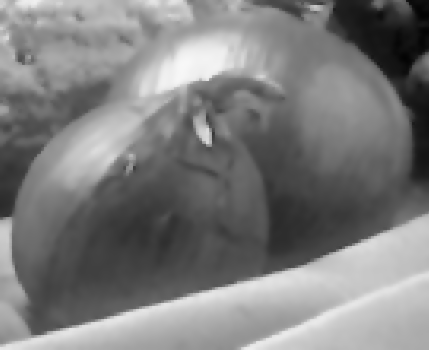
\includegraphics[width=4.5cm]{output_image/onion_ds3_rs50.png}
  \label{snack_onion_smooth}
  }
  \caption{The Bilater filtering result of snacks and the Onion detail}
  \label{snack}
\end{figure}


The Fig.~\ref{snack} presents the result of Bilateral filter (Fig.~\ref{snack_original_smooth}, ~\ref{snack_onion_smooth}) and their original images Fig.~\ref{snack_original} and \ref{snack_onion}.
The choosed parameter pair $(\sigma_d = 3$ and $\sigma_r = 50)$ is the same as paper mentioned.
As shown in Fig.~\ref{snack_original_smooth}, the salt and pepper noises can be removed.
Meanwhile, the edges can be preserved.
Fig.~\ref{snack_onion_smooth} is the detail of Fig.~\ref{snack_original_smooth}.


\subsubsection{Experiment result of color images}
\label{subsubsection color images}
The bilateral filter is not only suitable for filtering the gray image, but also achieving success for filtering color images.
In the paper, the author mentioned that transforming color space from RGB to CIE-lab color space can solve the color distorted problem directly dealing with RGB color space.

Fig.~\ref{color_child} has presented the result of filtering on color images with CIE-lab space.
Fig.~\ref{color_children_smooth} exhibits a similar result as printed on the paper.

Fig.~\ref{color} also presents some other noised images from the internet which can be smoothed and edge-keeping with Bilateral filtering.
In these images, the first row (Fig.~\ref{color_cube}, ~\ref{color_sky}, ~\ref{color_home}) are original images, and the second row (Fig.~\ref{color_cube_smooth}, ~\ref{color_sky_smooth} and~\ref{color_home_smooth}) are the smoothed result.

\begin{figure}[H]
  \centering
  \subfigure[Child]{
  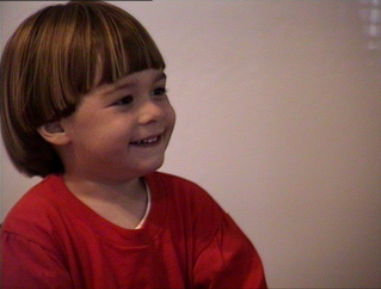
\includegraphics[width=6cm]{original_paper_images/color/child.png}
  \label{color_children}
  }
  \quad
  \subfigure[Smoothed Child]{
  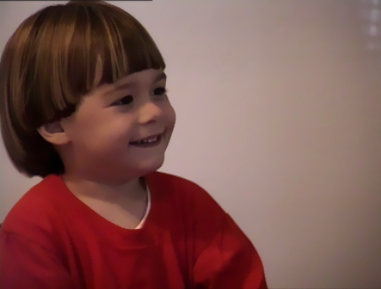
\includegraphics[width=6cm]{output_color_image/child_ds3_rs10.png}
  \label{color_children_smooth}
  }
  \caption{Output of child image}
  \label{color_child}
\end{figure}


\begin{figure}[H]
  \centering
  \subfigure[Rubik's cube]{
  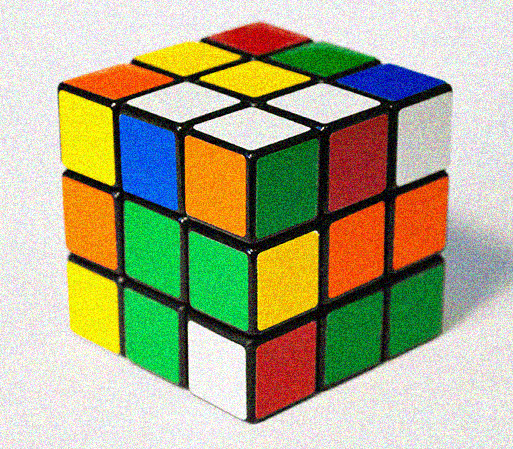
\includegraphics[width=4.5cm]{original_paper_images/color/rubiks_cube.png}
  \label{color_cube}
  }
  \quad
  \subfigure[Sky]{
  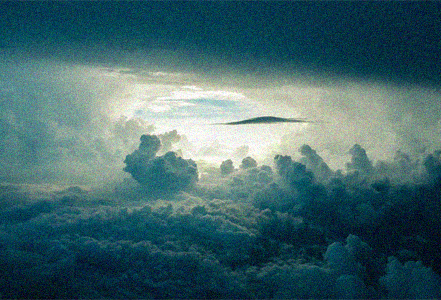
\includegraphics[width=4.5cm]{original_paper_images/color/sky.png}
  \label{color_sky}
  }
  \quad
    \subfigure[Home]{
    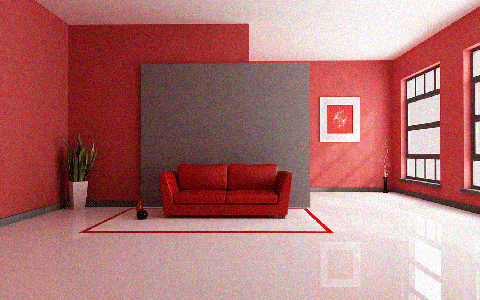
\includegraphics[width=4.5cm]{original_paper_images/color/home.png}
    \label{color_home}
    }
  \quad

  \subfigure[Smoothed Rubik's cube]{
  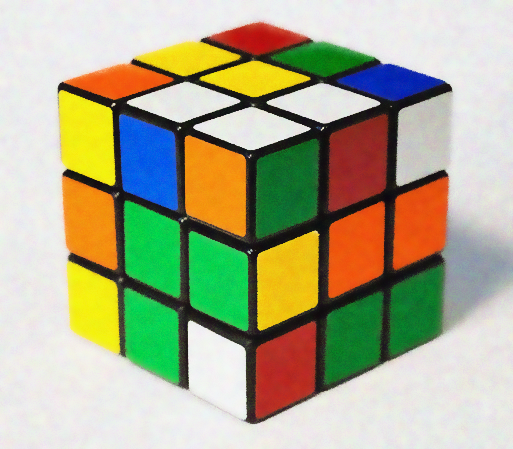
\includegraphics[width=4.5cm]{output_color_image/rubiks_cube_ds3_rs50.png}
  \label{color_cube_smooth}
  }
  \quad
  \subfigure[Smoothed sky]{
  \includegraphics[width=4.5cm]{output_color_image/sky_ds3_rs30.png}
  \label{color_sky_smooth}
  }
  \quad
  \subfigure[Smoothed home]{
  \includegraphics[width=4.5cm]{output_color_image/home_ds3_rs30.png}
  \label{color_home_smooth}
  }
  \caption{Outputs of other color images}
  \label{color}
\end{figure}

\subsection{Compare with other baseline algorithm}
\label{subsection baseline comparison}
In this section, we compared the results of the Bilateral filter with other baseline algorithms to present the advantages of our code.
Before the Bilateral filter, the gaussian filter is one of the useful methods which can smooth a noised image. 
Other low-pass filters, such as the Mean filter and Median filter will also be considered in our experiment. 
Since all of these filters are classic filtering methods in terms of image processing.

In the Section.~\ref{subsection reimplement}, our re-implement has proved the success of the Bilateral filtering method for gray and color images.
But only from the versioning aspect is not enough, sometimes, the human version may produce bias.

So, in our experiment, we use the quantitive method to compare our Bilateral filter output with different baseline low-pass filters with PNSR.
The equation of PNSR has been shown in Eq.~\ref{PSNR equation}.

\begin{equation}
  PSNR = 10\log 10 (\frac{I_{Max}^{2}}{MSE})
  \label{PSNR equation}
\end{equation}

\begin{equation}
  MSE = \frac{\sum_{M, N}[I_1(m,n) - I_2(m, n)]^2}{M * N}
  \label{MSE}
\end{equation}

Where the $I_{Max}$ is the maximum fluctuation in the input images. 
In our case, the 8-bit integer input image should have $I_{Max} = 255$.
And the $I_1$ and $I_2$ are the two images between the noisy and the filtered one.
  
\begin{figure}[H]
  \centering
  \subfigure[$Mean_{psnr}=19.89$]{
  \includegraphics[width=3.5cm]{output_baseline/cat_mean_23.png}
  \label{gray_baseline_mean}
  }
  \quad
  \subfigure[$Median_{psnr}=20.66$]{
  \includegraphics[width=3.5cm]{output_baseline/cat_median_23.png}
  \label{gray_baseline_median}
  }
  \quad
  \subfigure[Gaussian $\sigma=1$]{
  \includegraphics[width=3.5cm]{output_baseline/cat_gaussian_23_ds_1.png}
  \label{gray_baseline_gaussian1}
  }
  \quad

  \subfigure[Gaussian $\sigma=3$]{
  \includegraphics[width=3.5cm]{output_baseline/cat_gaussian_23_ds_3.png}
  \label{gray_baseline_gaussian3}
  }
  \quad
  \subfigure[Gaussian $\sigma=10$]{
  \includegraphics[width=3.5cm]{output_baseline/cat_gaussian_23_ds_10.png}
  \label{gray_baseline_gaussian10}
  }
  \quad
  \subfigure[Bilateral filter output]{
  \includegraphics[width=3.5cm]{output_image/cat_ds10_rs10.png}
  \label{gray_baseline_bilateral}
  }
  \caption{output compared with the baseline low pass filters in gray scale}
  \label{gray_baseline}
\end{figure}


Fig.~\ref{gray_baseline} has presented the result between three baseline filters and the Bilateral filter. 
It is obvious that Fig.~\ref{gray_baseline_mean} and Fig.~\ref{gray_baseline_median} get bad results, due to the reason that all the details and texture information are lost. 
The only remaining parts are the contour of the cat in each image.
The result of Gaussian filter, as shown in Fig.~\ref{gray_baseline_gaussian1}, ~\ref{gray_baseline_gaussian3}, ~\ref{gray_baseline_gaussian10}, indicates that the smaller $\sigma$ of gaussian filter achieves better result. 
However, with the increase of the $sigma$ values, the result of the gaussian filter gets fuzzy.
The Fig.~\ref{gray_baseline_gaussian1} and Fig.~\ref{gray_baseline_bilateral} prove the statement in \cite{paper_bf}.
Gaussian blur will also smooth the edges, in Fig.~\ref{gray_baseline_gaussian1}, the whiskers of the cat also become fuzzy, but still maintains clear in Fig.~\ref{gray_baseline_bilateral}.

Table.~\ref{table_PSNR_gray} presents the PSNR result. 
As the result in the table, gaussian blur have some lower scores when $\sigma$ = $sigma_d$ in Bilateral filtering.
The PSNR score of Gaussian close the score of the Bilateral filter when $\sigma_r = 300$.
But for each $sigma_d = (1, 3, 10)$, the most ambiguous result is obtained when $sigma_r= 300$.


\begin{table}[H]
\centering
\begin{tabular}{lllll}
\cline{1-5}
Method & Kernel\_size & sigma\_s & Sigma\_r & PSNR  \\ \cline{1-1}
\cline{1-5}
\multirow{4}{*}{Bilateral Filter}   & \multirow{4}{*}{23} & \multirow{4}{*}{1}                               
                                  & 10      & 42.74 \\
       &             &            & 30      & 36.26     \\
       &             &            & 100     & 32.59     \\
       &             &            & 300     & 31.70     \\
\cline{1-5}
Gaussian filter($\sigma = 1$)    & 23    &      &       & 31.59    \\
\cline{1-5}
\multirow{4}{*}{Bilateral Filter}   & \multirow{4}{*}{23} & \multirow{4}{*}{3}  
                                  & 10       &40.05     \\
      &              &            & 30       & 31.37     \\
      &              &            & 100      & 25.90     \\
      &              &            & 300      & 24.39     \\
\cline{1-5}   
Gaussian filter($\sigma = 3$)    & 23    &      &     & 24.13\\    
\cline{1-5}                        
\multirow{4}{*}{Bilateral Filteral} & \multirow{4}{*}{23} & \multirow{4}{*}{10} 
                                  & 10       & 39.59     \\
     &               &            & 30       & 29.74     \\
     &               &            & 100      & 22.57     \\
     &               &            & 300      & 20.69     \\
\cline{1-5}
Gaussian filter($\sigma = 10$)    & 23    &      &       & 20.41\\
\cline{1-5}
\end{tabular}
\caption{The PSNR output for gray image}
\label{table_PSNR_gray}
\end{table}

The same situation also happened filtering color images.
Fig.~\ref{color_baseline} indicates that the Mean and Median blur can only maintain a contour of the object and the Gaussian filter with $\sigma = 1$ achieves the clearest output in all the Gaussian filters. 
It is apparent that the Bilateral filter has the highest result as shown in Table.~\ref{table_PSNR_color}.

\begin{figure}[H]
  \centering
  \subfigure[$Mean_{psnr}=26.12$]{
  \includegraphics[width=3.5cm]{output_baseline/child_mean_23.png}
  \label{color_baseline_mean}
  }
  \quad
  \subfigure[$Median_{psnr}=28.59$]{
  \includegraphics[width=3.5cm]{output_baseline/child_median_23.png}
  \label{color_baseline_median}
  }
  \quad
  \subfigure[Gaussian $\sigma=1$]{
  \includegraphics[width=3.5cm]{output_baseline/child_gaussian_23_ds_1.png}
  \label{color_baseline_gaussian1}
  }
  \quad

  \subfigure[Gaussian $\sigma=3$]{
  \includegraphics[width=3.5cm]{output_baseline/child_gaussian_23_ds_3.png}
  \label{color_baseline_gaussian3}
  }
  \quad
  \subfigure[Gaussian $\sigma=10$]{
  \includegraphics[width=3.5cm]{output_baseline/child_gaussian_23_ds_10.png}
  \label{color_baseling_gaussian10}
  }
  \quad
  \subfigure[Bilateral filter]{
  \includegraphics[width=3.5cm]{output_color_image/child_ds3_rs10.png}
  \label{color_baseline_bilateral}
  }
  \caption{output compared with the baseline low pass filters in color iamges}
  \label{color_baseline}
\end{figure}

%------------compare with this baseline filter

\begin{table}[H]
  \centering
  \begin{tabular}{lllll}
  \cline{1-5}
  Method & Kernel\_size & sigma\_s & Sigma\_r & PSNR  \\ \cline{1-1}
  \cline{1-5}
  \multirow{4}{*}{Bilateral Filter}   & \multirow{4}{*}{23} & \multirow{4}{*}{1}                               
                                    & 10      & 42.91 \\
         &             &            & 30      & 41.22     \\
         &             &            & 100     & 39.42     \\
         &             &            & 300     & 38.96     \\
  \cline{1-5}
  Gaussian filter($\sigma = 1$)      & 23 &  & & 39.01     \\
  \cline{1-5}
  \multirow{4}{*}{Bilateral Filter}   & \multirow{4}{*}{23} & \multirow{4}{*}{3}  
                                    & 10       &39.02    \\
        &              &            & 30       &35.92   \\
        &              &            & 100      &32.35    \\
        &              &            & 300      &31.19     \\
  \cline{1-5}     
  Gaussian filter($\sigma = 3$)  & 23 &  & & 31.11 \\
  \cline{1-5}                            
  \multirow{4}{*}{Bilateral Filteral} & \multirow{4}{*}{23} & \multirow{4}{*}{10} 
                                    & 10       & 39.27    \\
       &               &            & 30       & 33.18     \\
       &               &            & 100      & 28.46    \\
       &               &            & 300      & 26.86     \\
  \cline{1-5}
  Gaussian filter($\sigma = 10$)     & 23 &  & & 26.73  \\
  \cline{1-5}  
\end{tabular}
\caption{The PSNR output for color image}
\label{table_PSNR_color}
\end{table}





\section{Conclusion}
\label{section conclusion}
In a conclusion, in this report, we successfully re-implement the Bilateral filter based on the guidance of the content mentioned in ~\cite{paper_gabf}.
We have proved that Bilateral filter can optimize better compared with other low-pass filters. 
Especially it reduce the negative impact on the blured edges by Gaussian filter.
We also explored the quality of outputs between Bilateral filtering and other low-pass filters.
By presentt the reuslt of this, we quantitively analyzed the performance of Bilateral filter by evaluating PSNR score between difference filters.


However, there are some drawbacks to our re-implement. 
Firstly, the Bilateral filter is a brute-force loop calculating algorithm, as it searches all the pixels from an input image.
Without any search optimization of our re-implement code, the calculation will become slower when the input image size becomes large or the kernel size increase.
Secondly, the evaluation method we chose is not the best one for evaluating blured pictures
PSNR values sometimes do not match the visual quality perceived by the human eye, such as the PSNR does not represent the visual perceptual properties of the human eye well~\cite{paper_psnr}.
Also, PSNR is not sensitive to structural changes when blurring occurs.  
Based on this, PSNR has some limitations, it may not correctly reflect the result in some cases.

Not only the Bilateral filter,there are also many knowledges we take advantages of class.
The first is PSNR, as mentioned before, we use this as an evaluation indicator to quantitive evaluate our re-implement output and other baseline low-pass filters.
Also, The low-pass filters we choose, such as mean, median, and gaussian are all introduced in class.
especially, we further explore the properties of the Gaussian filter and understand its advantage and drawbacks respectively.
Besides, during the re-implement process, we also utilize the padding method explained in the class. 
The zero-padding is a easy method but not the optimal choice, so, in the end, we choose the reflection padding as our pre-processing.


There are also some difficulties during our implementation process.
The first is the omission parameters in the original paper.
The original paper lacked information about the chosen of kernel size. 
Also, since this article was published 20 years ago, finding the images used by the author at that time was a very difficult task. 
The resolution ratios of these images from the internet or cut from paper are different.
Different resolution ratios not only influence the output result, also impact the choice of experiment parameters.
These difficulties spent us a huge amount of time to figure out the solution.

\end{document}
